\documentclass{article}
\newcommand{\fullwidth}{18.875in} % including edge bleed on both sides
\newcommand{\fullheight}{8.25in}  % including edge bleed on top and bottom
% Bookmobile Template widths.  Set these according to the template
\newcommand{\trim}{0.125in}
\newcommand{\flap}{3in}
\newcommand{\wrap}{0.188in}
\newcommand{\cover}{6in}
\newcommand{\spine}{0.25in}
% Order: trim flap wrap cover spine cover wrap flap trim

% These are calculated from the above
\newlength{\Xlogo}
% Change the Xmm to move the item relative to it's default position

\usepackage[paperwidth=\fullwidth,paperheight=\fullheight,margin=0in]{geometry}
\usepackage{graphicx}
%\usepackage[colorgrid,texcoord]{eso-pic}[2002/11/16] % FOR THE GRID
\usepackage{calc}
%\usepackage[showboxes,absolute]{textpos}
\usepackage[absolute]{textpos}
\usepackage{bold-extra}
\usepackage{tikz}
\usepackage{color}
\usepackage{tgbonum}
\usepackage{pdfpages}
\setlength{\TPHorizModule}{1in}
\setlength{\TPVertModule}{1in}
\definecolor{AuthorColor}{rgb}{1 1 1}
\definecolor{TitleColor}{rgb}{1 1 1  }
\definecolor{RColor}{rgb}{.8 .8 .8}


% These are calculated from the above.  The non-symbolic quantity can be used
% for relative positioning of the item


% ISBN 978-0-9839658-9-3
\begin{document}
\setlength{\Xlogo}{\trim+\flap+\wrap+7mm}
%%%% Cover Main Part
\begin{textblock}{6.188}(3.125,0)
\noindent\begin{tikzpicture}
%\fill[white,opacity=.2] (0in,-8.25in) rectangle (12.81in,0in); 
\end{tikzpicture}
\end{textblock}

%%%% Back Cover Contents
\begin{textblock*}{5}(3.5in,.6in) 
\parbox{130mm}{

\textsc{\bfseries{A Student Reference for Statistics Using R}} is one
of a series of books designed to help statistics educators master
integrating modern computation in their courses. We refer to our
approach as {\bf computational statistics} because
the availability of computation is shaping how statistics is done,
taught, and understood. Computational statistics is a key component of
{\bf data science}, using data to answer questions and communicate
results. 

\noindent Other books in the series include:
\begin{itemize}
\setlength\itemsep{0mm}
\item \textsc{Start Modeling with R}
\item \textsc{Start Teaching with R}
\item \textsc{Start R in Calculus}
\end{itemize}


These materials have been shared with hundreds of statistics educators
through workshops run under the auspices of Project Mosaic, CAUSE, the
Mathematical Association of America, the American Statistical
Association, the W.M. Keck Foundation, the Howard Hughes Medical
Institute, and the US National
Science Foundation. 


\raggedright
\noindent \noindent {\bf Nicholas Horton}, {\bf Randall Pruim}, and {\bf
Daniel Kaplan} teach statistics, mathematics, and computation at
Amherst College, Calvin College, and Macalester College
respectively.  They are co-PIs on the National Science Foundation
support Project MOSAIC (NSF DUE-0920350).

\medskip

\centerline{\begin{tabular}{ccc}
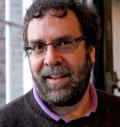
\includegraphics[height=1in]{../../CoverImages/horton.jpg} & 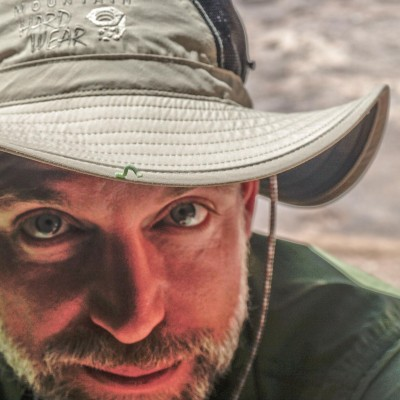
\includegraphics[height=1in]{../../CoverImages/pruim.jpg} & 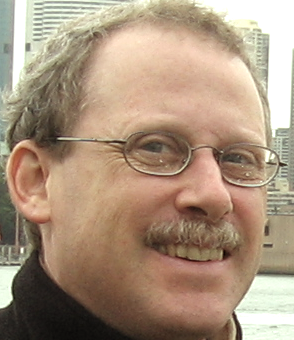
\includegraphics[height=1in]{../../CoverImages/kaplan.png}\\
{\sc Horton} & {\sc Pruim} & {\sc Kaplan}\\
\end{tabular}}

\medskip

\noindent {\bf Other books by the authors:}\\
{\em Using R for Data Management, Statistical Analysis and Graphics} (NJH \& KK)\\
{\em Foundations and Applications of Statistics: An Introduction Using
  R } (RJP), {\em Gems of Theoretical Computer Science} (US \& RJP),
{\em Understanding Nonlinear Dynamics} (DTK), {\em Statistical Modeling: A Fresh Approach} (DTK), {\em Start R in Calculus} (DTK)
}
\end{textblock*} 

\begin{textblock}{4}(3.5,.5)
\noindent\begin{tikzpicture}
\fill [white,opacity=.75] (0in,-6.1in) rectangle (5.4in,0in);
\end{tikzpicture}
\end{textblock}

%%%% Front Cover Lightener
\begin{textblock}{6.188}(9.55,0) % moved 0.25 from 9.3
\noindent\begin{tikzpicture}
% \fill [white,opacity=.3] (0in,-8.25in) rectangle (6.881in,0in);
\end{tikzpicture}
\end{textblock}


%%%% Title

%%%% Title

\begin{textblock*}{5.2}(237mm,1.8in) %8.6
\noindent{%
\hbox{\parbox{4.5in}{\noindent\raggedleft{\textsc{\bfseries{%
\fontsize{28pt}{60pt}\selectfont\textcolor{TitleColor}{%
\hfill A Student Reference for \newline \hspace{0pt} \newline\hspace{0pt}{\tiny .}\hfill
Commands to Teach%
\newline \hspace{0pt} \newline\hfill Statistics with }}}}}\bfseries{{\fontsize{150pt}{60pt}\selectfont\textcolor{RColor}{\raisebox{-.75in}{R}}}}}}
\end{textblock*}

\begin{textblock*}{4.5in}(285mm,5in) 

\noindent{\textsc{\bfseries{\fontsize{22pt}{60pt}\selectfont
     \textcolor{AuthorColor}{Nicholas J. Horton\\\\Randall Pruim\\\\Daniel T. Kaplan}}}}
\end{textblock*}

% Spine New

\begin{textblock*}{\spine}(\trim+\flap+\wrap+\cover+\spine/2 + 7pt,0) % was 9.44

\vspace*{.4in}

\noindent\hspace{-.2in}\rotatebox{270}{\large\bf
  \textcolor{yellow}{A Student Reference for Statistics Using R}
    \hspace{.3in}Horton, Pruim, Kaplan
  \hspace{.3in}{\textcolor{yellow}{\sf Project MOSAIC}}\hspace*{.25in}\raisebox{-1.3mm}{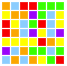
\includegraphics[width=0.21in]{../../CoverImages/mosaic-square.png}}}
\end{textblock*}

%%% Logos
\begin{textblock*}{1.5}(\Xlogo,6.65in)  
\noindent
\includegraphics[width=1.5in]{../../CoverImages/mosaic-logo-small.png}
\medskip
\noindent \rule{2pt}{0pt}
\includegraphics[width=1.425in]{../../CoverImages/RStudio.png}
\end{textblock*}


%%% ISBN 978-0-9839658-6-2
\begin{textblock}{1.65}(6.6,6.85)   % Same as above
\noindent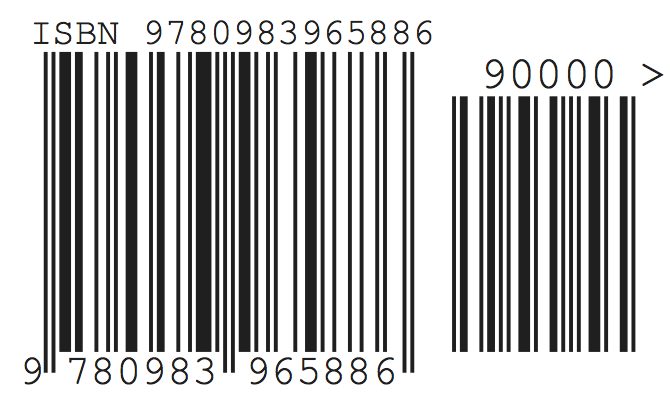
\includegraphics[width=1.75in]{../../CoverImages/ISBN-8-6.png}
\end{textblock}
\begin{textblock}{1.65}(6.6,6.85)
\noindent\begin{tikzpicture}
\fill [white,opacity=.75] (-1.75in,-1in) rectangle (0in,0in);
\end{tikzpicture}
\end{textblock}


%% Back Flap

\begin{textblock*}{3}(\trim,.25in)
\noindent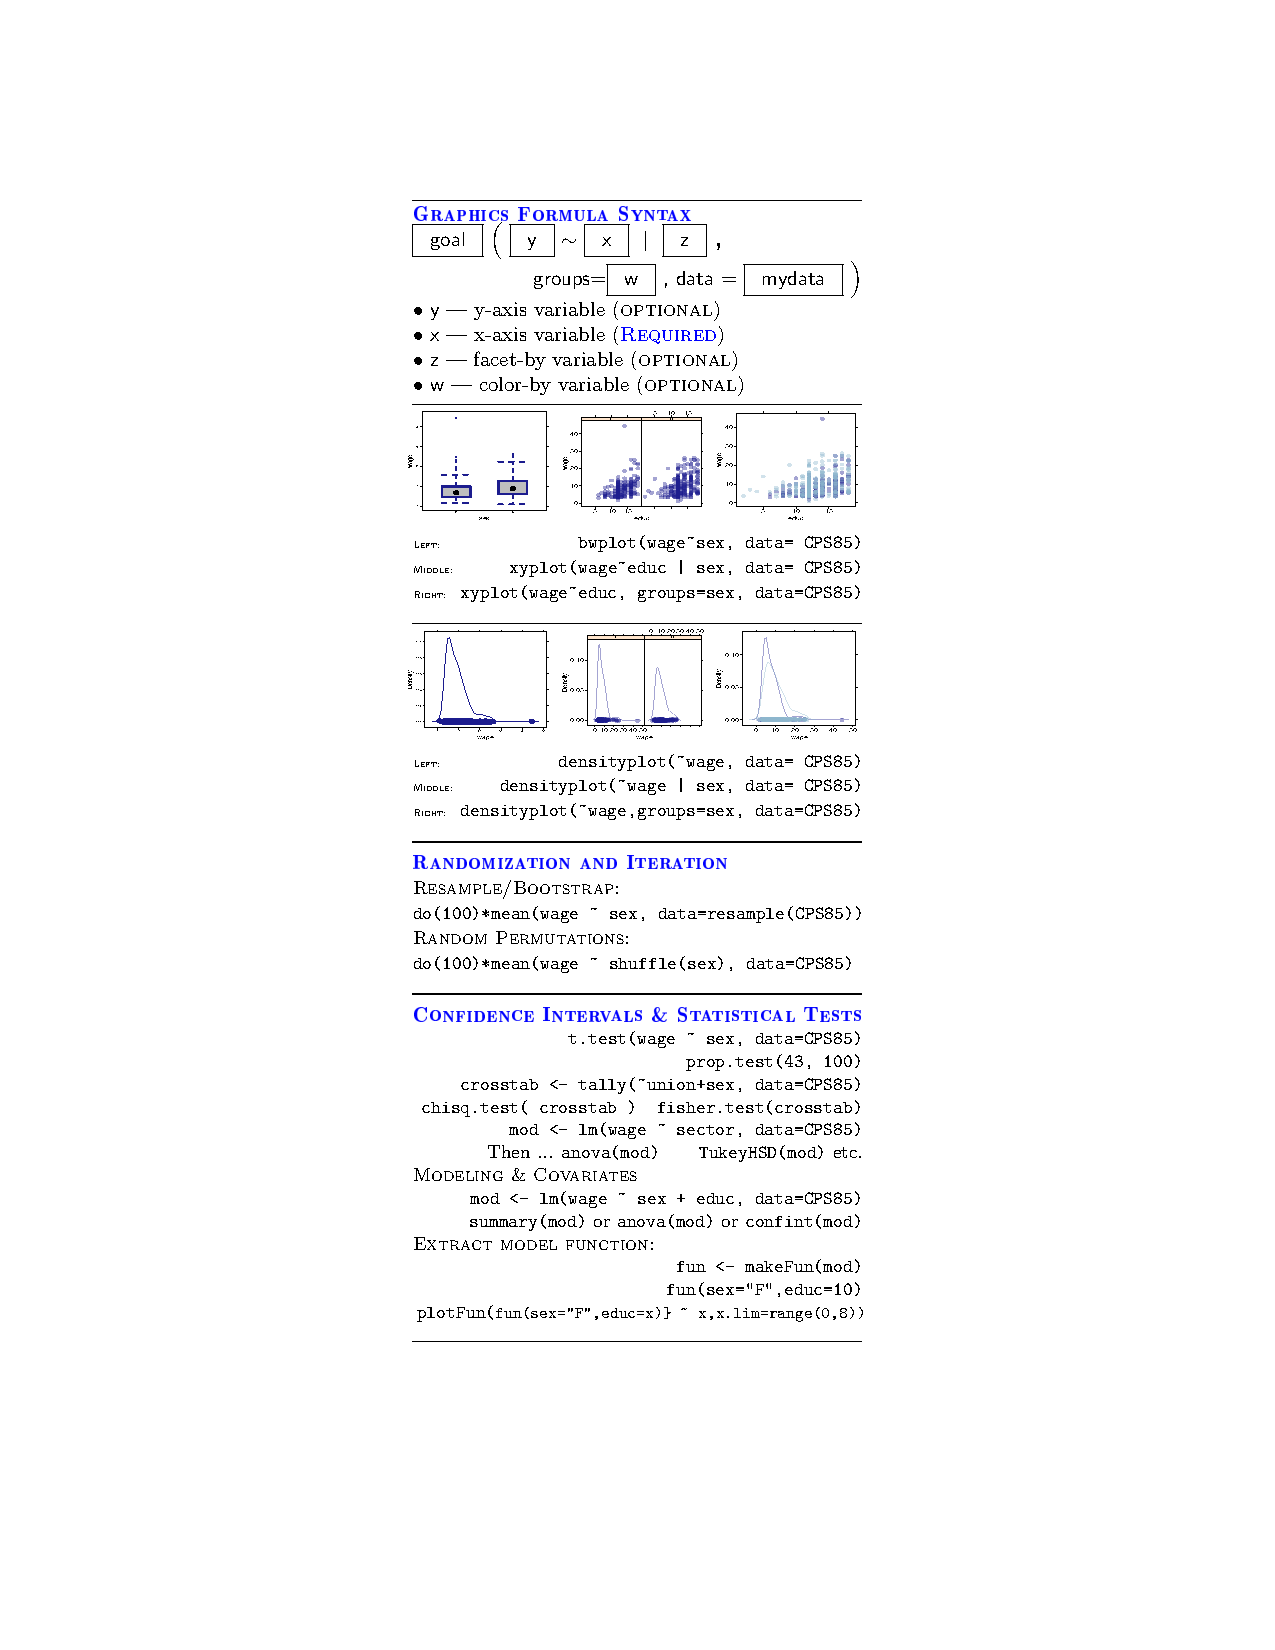
\includegraphics[width=2.9in]{backflap.pdf}
\end{textblock*}

\begin{textblock}{3}(0,0)
\noindent\begin{tikzpicture}
\fill [white,opacity=.75] (0in,0in) rectangle (3.1in,8.4in);
\end{tikzpicture}
\end{textblock}

% Front Flap

\begin{textblock*}{3}(\trim+\flap+\wrap+\cover+\spine+\cover+\wrap-2mm,.25in) % 15.73
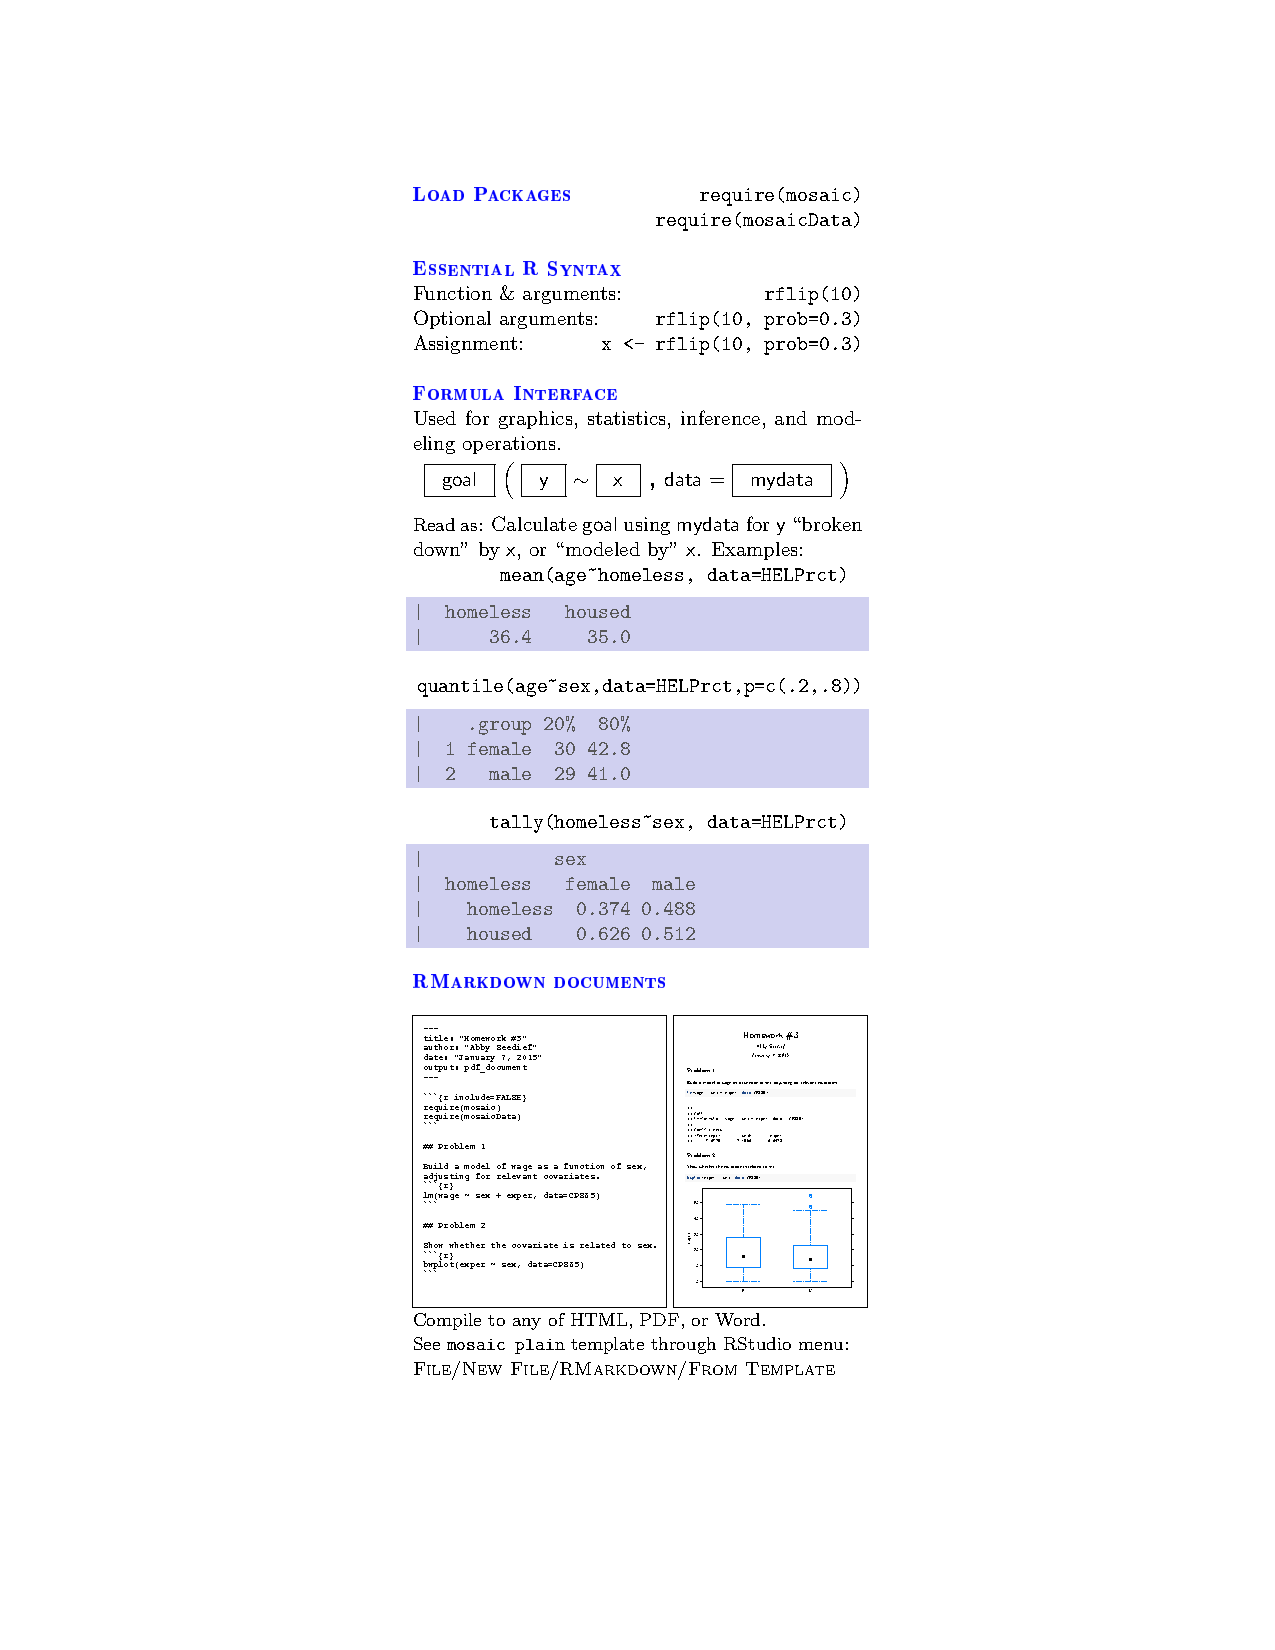
\includegraphics[width=2.9in]{frontflap.pdf}
\end{textblock*}

\begin{textblock*}{3}(\trim+\flap+\wrap+\cover+\spine+\cover+\wrap,0) % was 15.9
\noindent\begin{tikzpicture}
\fill [white,opacity=.75] (0in,0in) rectangle (3.125in,8.25in);
\end{tikzpicture}
\end{textblock*}

% Front Photo
\begin{textblock}{6.125}(9.3,0)
\noindent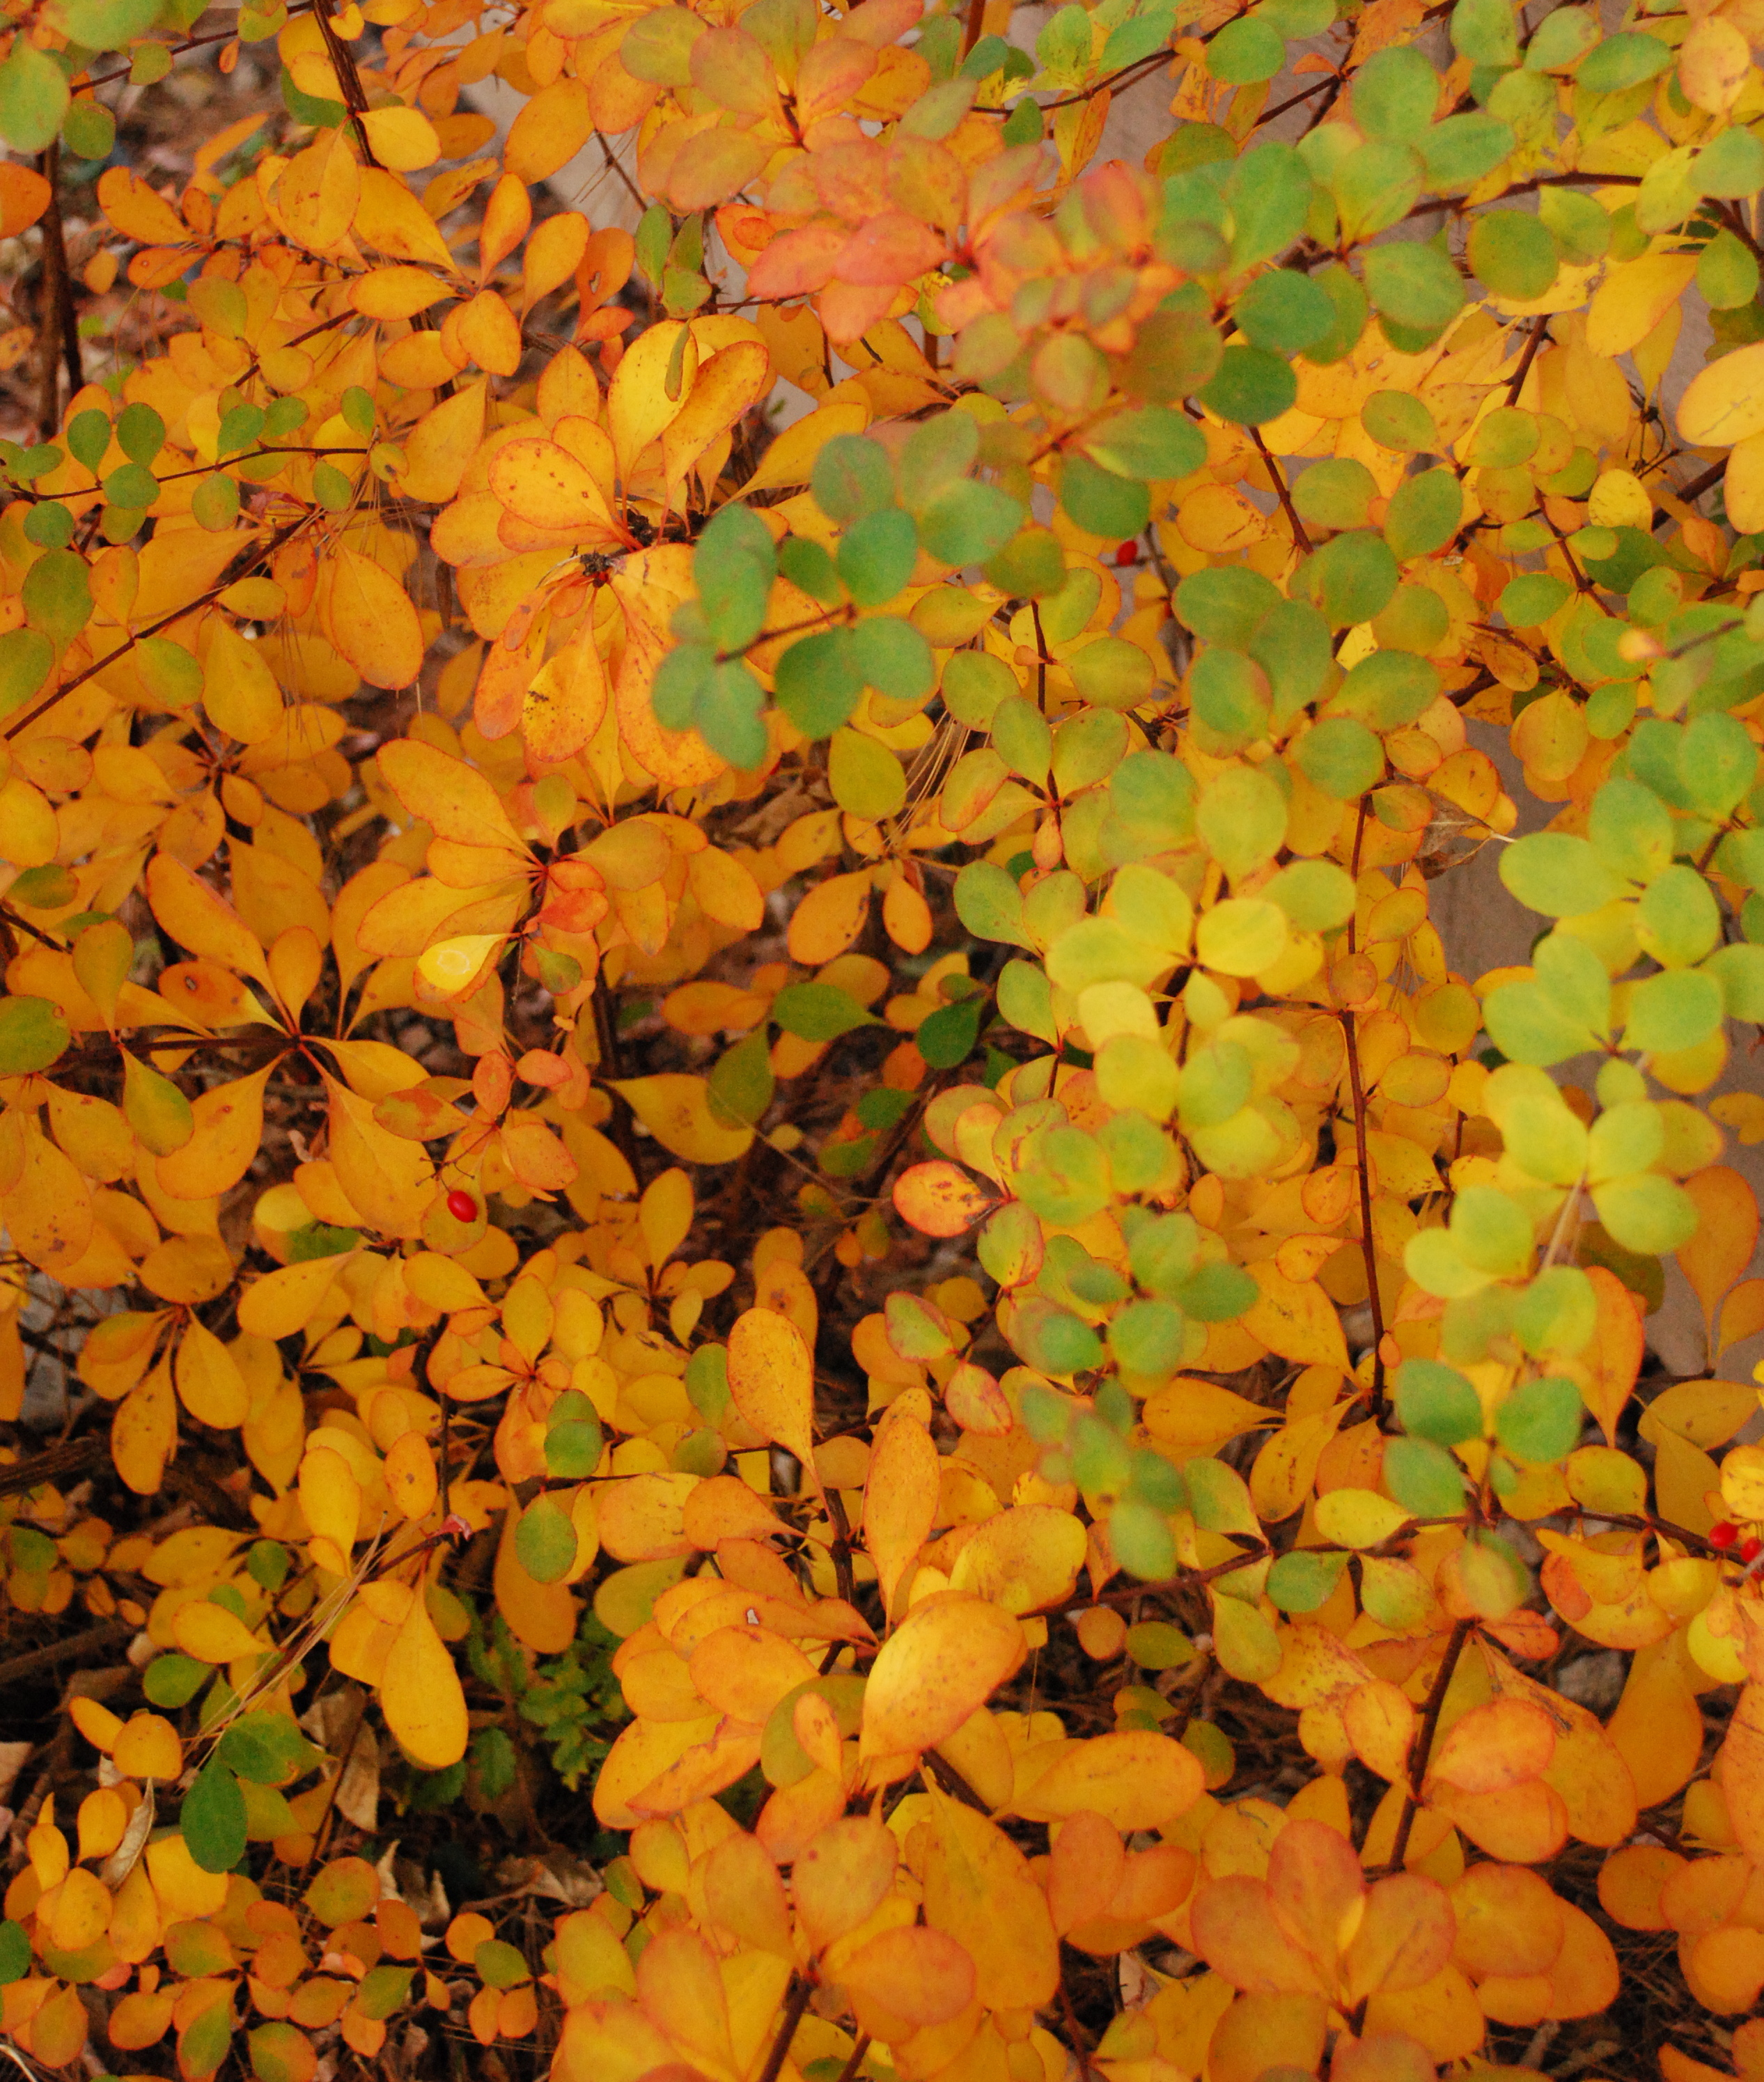
\includegraphics[angle=90,height=8.25in,width=9.881in]{../../CoverImages/FrontMain.jpg}
\end{textblock}

% Back Photo
\begin{textblock}{6.125}(-0.2,0)
\noindent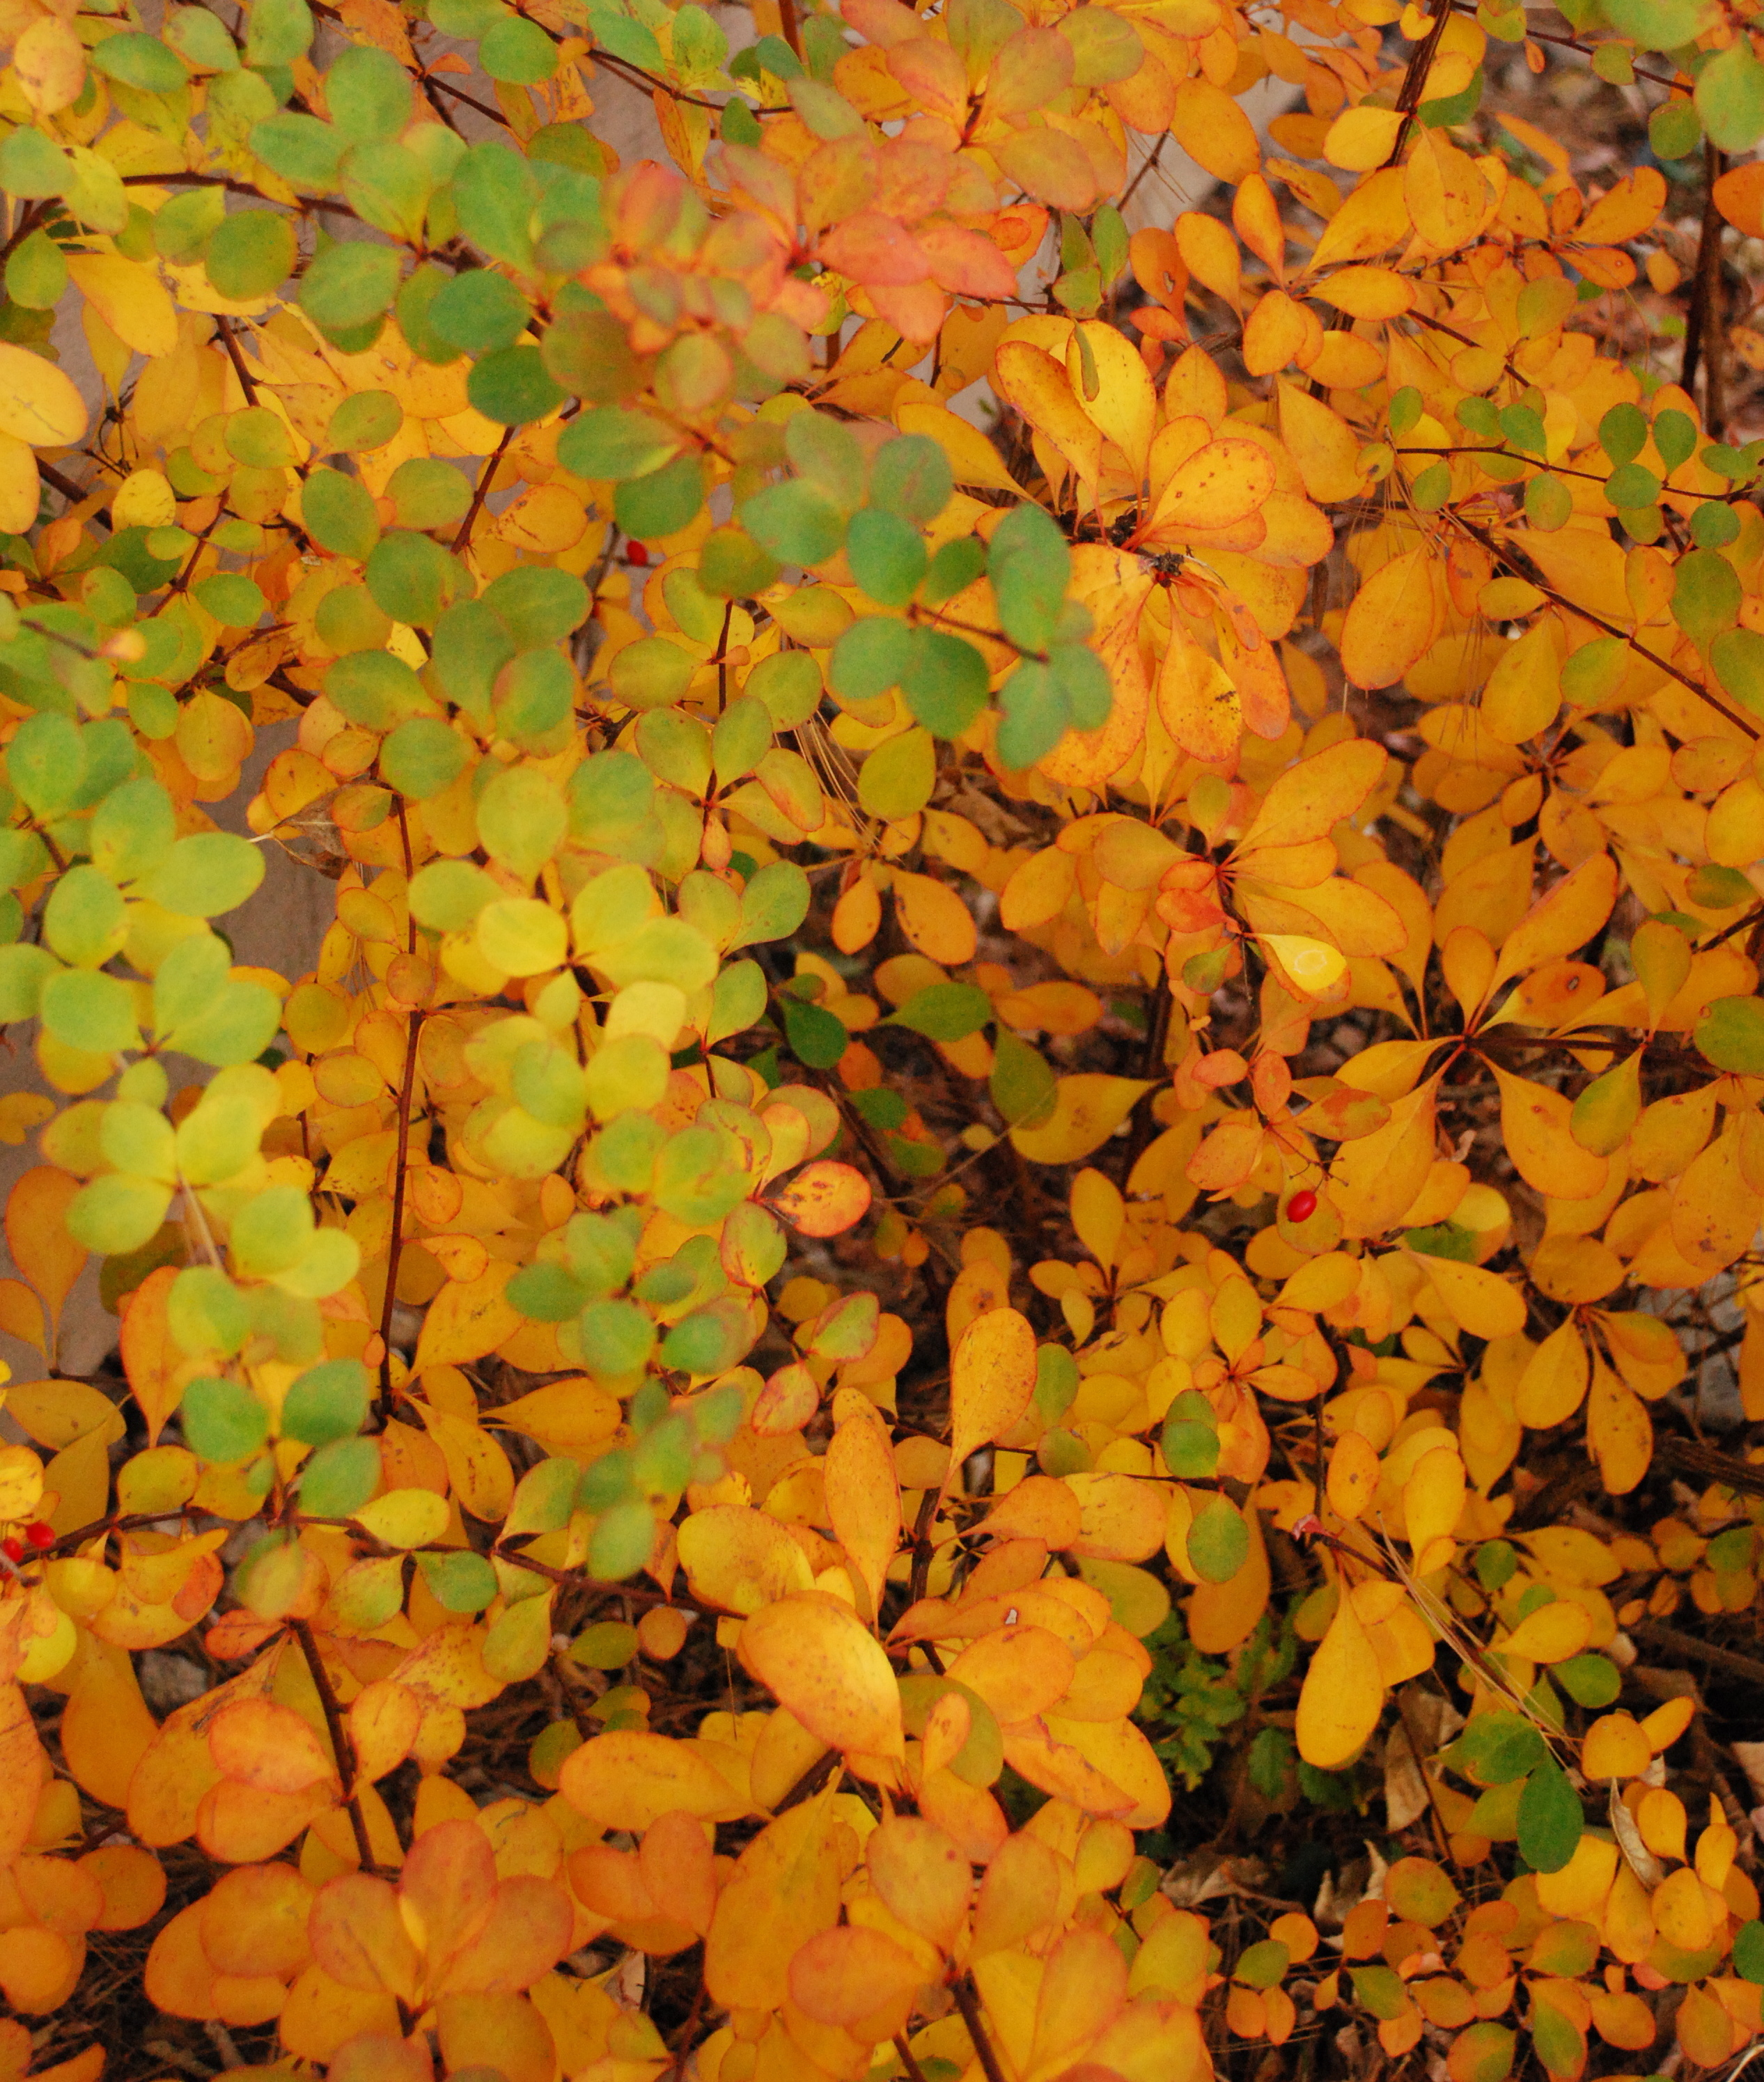
\includegraphics[angle=90,height=8.25in,width=9.881in]{../../CoverImages/BackMain.jpg}
\end{textblock}


\end{document}

